\chapter{Tutorial}
\section{Bloques}
\subsection{Definición}
\subsubsection{Definición sin referencia }
\defn{Nombre de la definición}{\lipsum[1]}
\subsubsection{Definición con referencia}
\defnr{Nombre de la definición con referencia}{nombre_de_referencia}{\lipsum[1] }

\subsection{Suposición}
\subsubsection{Suposición sin referencia}
\supos{}{\lipsum[1]}
\subsubsection{Suposición con referencia}
\suposr{}{}{\lipsum[1]}
\newpage

\subsection{Teorema}
\subsubsection{Teorema sin referencia}
\teo{}{\lipsum[1]}
\subsubsection{Teorema con referencia y demostración}
\teor{}{}{\lipsum[1]}
\begin{teop}
    \lipsum[1]
\end{teop}

\subsection{Lema}
\subsubsection{Lema sin referencia}
\lem{}{\lipsum[1]}
\subsubsection{Lema con referencia y demostración}
\lemr{}{}{\lipsum[1]}
\begin{lemp}
    \lipsum[1]
\end{lemp}

\subsection{Corolario}
\subsubsection{Corolario sin referencia}
\cor{}{\lipsum[1]}
\subsubsection{Corolario con referencia y demostración}
\corr{}{}{\lipsum[1]}
\begin{corp}
    \lipsum[1]
\end{corp}

\subsection{Proposición}
\subsubsection{Proposición sin referencia}
\prop{}{\lipsum[1]}
\subsubsection{Proposición con referencia y demostración}
\propr{}{}{\lipsum[1]}
\begin{propp}
    \lipsum[1]
\end{propp}

\subsection{Proposición}
\subsubsection{Proposición sin referencia}
\prop{}{\lipsum[1]}
\subsubsection{Proposición con referencia y demostración}
\propr{}{}{\lipsum[1]}
\begin{propp}
    \lipsum[1]
\end{propp}

\subsection{Afirmación}
\subsubsection{Afirmación sin referencia}
\af{}{\lipsum[1]}
\subsubsection{Afirmación con referencia y demostración}
\afr{}{}{\lipsum[1]}
\begin{afp}
    \lipsum[1]
\end{afp}

\subsection{Hecho}
\he{}{}{\lipsum[1]}
\newpage
\subsection{Ejemplo}
\subsubsection{Ejemplo sin referencia}
\ej{}{\lipsum[1]}
\subsubsection{Ejemplo con referencia y demostración}
\ejr{}{}{\lipsum[1]}
\begin{ejp}
    \lipsum[1]
\end{ejp}

\subsection{Hecho}
\he{}{}{\lipsum[1]}
\newpage

\subsection{Observación}
\subsubsection{Observación sin referencia}
\ob{}{\lipsum[1]}
\subsubsection{Observación con referencia y demostración}
\obr{}{}{\lipsum[1]}
\begin{obp}
    \lipsum[1]
\end{obp}
\newpage

\section{Figuras}
\subsection{Una sola figura}
\begin{figure}[H]
	\centering
	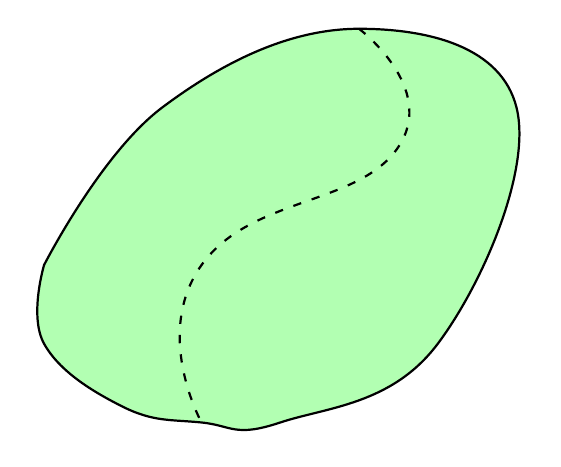
\begin{tikzpicture}
		\fill[green!30] 
		plot[smooth, tension=0.7] coordinates {
			(0,0)
			(1.5,2)
			(4,3)
			(6,2)
			(5,-1)
			(3,-2)
			(2,-2)
			(1,-1.8)
			(0,-1)
			(0,0)
		};
		
		\draw[thick, black] 
		plot[smooth, tension=0.7] coordinates {
			(0,0)
			(1.5,2)
			(4,3)
			(6,2)
			(5,-1)
			(3,-2)
			(2,-2)
			(1,-1.8)
			(0,-1)
			(0,0)
		};
		
		\draw[dash pattern=on 3pt off 4pt, thick, black] 
		plot[smooth, tension=0.9] coordinates {
			(4,3)
			(4.5,1.5)
			(2,0)
			(2,-2)
		};
	\end{tikzpicture}
	\caption{Ejemplo 1 de figura}
	\label{fig:1_00a}
\end{figure}

\begin{figure}[H]
	\centering
	\begin{tikzpicture}
		% Functions i
		\path[->] (0.8, 0) edge [bend right] node[left, xshift=-2mm] {$\phi_i$} (-1, -2.9);
		\draw[white,fill=white] (0.06,-0.57) circle (.15cm);
		\path[->] (-0.7, -3.05) edge [bend right] node [right, yshift=-3mm] {$\phi^{-1}_i$} (1.093, -0.11);
		\draw[white, fill=white] (0.95,-1.2) circle (.15cm);
		
		% Functions j
		\path[->] (5.8, -2.8) edge [bend left] node[midway, xshift=-5mm, yshift=-3mm] {$\phi^{-1}_j$} (3.8, -0.35);
		\draw[white, fill=white] (4,-1.1) circle (.15cm);
		\path[->] (4.2, 0) edge [bend left] node[right, xshift=2mm] {$\phi_j$} (6.2, -2.8);
		\draw[white, fill=white] (4.54,-0.12) circle (.15cm);
		
		% Manifold
		\draw[smooth cycle, tension=0.4, fill=white, pattern color=brown, pattern=north west lines, opacity=0.7] plot coordinates{(2,2) (-0.5,0) (3,-2) (5,1)} node at (3,2.3) {$M$};
		
		% Help lines
		%\draw[help lines] (-3,-6) grid (8,6);
		
		% Subsets
		\draw[smooth cycle, pattern color=orange, pattern=crosshatch dots] 
		plot coordinates {(1,0) (1.5, 1.2) (2.5,1.3) (2.6, 0.4)} 
		node [label={[label distance=-0.3cm, xshift=-2cm]:$U_i$}] {};
		\draw[smooth cycle, pattern color=blue, pattern=crosshatch dots] 
		plot coordinates {(4, 0) (3.7, 0.8) (3.0, 1.2) (2.5, 1.2) (2.2, 0.8) (2.3, 0.5) (2.6, 0.3) (3.5, 0.0)} 
		node [label={[label distance=-0.8cm, xshift=.75cm, yshift=1cm]:$U_j$}] {};
		
		% First Axis
		\draw[thick, ->] (-3,-5) -- (0, -5) node [label=above:$\phi_i(U_i)$] {};
		\draw[thick, ->] (-3,-5) -- (-3, -2) node [label=right:$\mathbb{R}^m$] {};
		
		% Arrow from i to j
		\draw[->] (0, -3.85) -- node[midway, above]{$\psi_{ij}$} (4.5, -3.85);
		
		% Second Axis
		\draw[thick, ->] (5, -5) -- (8, -5) node [label=above:$\phi_j(U_j)$] {};
		\draw[thick, ->] (5, -5) -- (5, -2) node [label=right:$\mathbb{R}^m$] {};
		
		% Sets in R^m
		\draw[white, pattern color=orange, pattern=crosshatch dots] (-0.67, -3.06) -- +(180:0.8) arc (180:270:0.8);
		\fill[even odd rule, white] [smooth cycle] plot coordinates{(-2, -4.5) (-2, -3.2) (-0.8, -3.2) (-0.8, -4.5)} (-0.67, -3.06) -- +(180:0.8) arc (180:270:0.8);
		\draw[smooth cycle] plot coordinates{(-2, -4.5) (-2, -3.2) (-0.8, -3.2) (-0.8, -4.5)};
		\draw (-1.45, -3.06) arc (180:270:0.8);
		
		\draw[white, pattern color=blue, pattern=crosshatch dots] (5.7, -3.06) -- +(-90:0.8) arc (-90:0:0.8);
		\fill[even odd rule, white] [smooth cycle] plot coordinates{(7, -4.5) (7, -3.2) (5.8, -3.2) (5.8, -4.5)} (5.7, -3.06) -- +(-90:0.8) arc (-90:0:0.8);
		\draw[smooth cycle] plot coordinates{(7, -4.5) (7, -3.2) (5.8, -3.2) (5.8, -4.5)};
		\draw (5.69, -3.85) arc (-90:0:0.8);
		
	\end{tikzpicture}
	\caption{Ejemplo 2 de figura}
	\label{fig:1_00b}
\end{figure}

\begin{figure}[H]
	\centering
	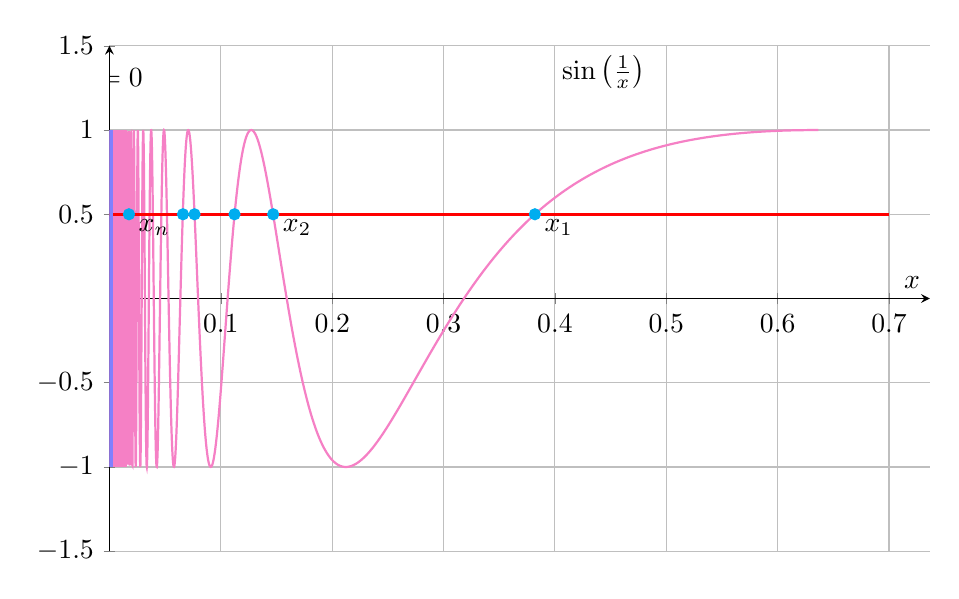
\begin{tikzpicture}
		\begin{axis}[
				domain=0.015:2/pi, % Intervalo de x
				samples=5000, % Número de muestras para mayor precisión
				xlabel={$x$},
				ylabel={$\qquad \qquad \qquad \qquad \qquad \qquad \qquad \qquad \sin\left(\frac{1}{x}\right)$},
				grid=both,
				width=12cm,
				height=8cm,
				axis lines=middle,
				ymin=-1.5, ymax=1.5,
				xmin=0, xmax=2/pi + 0.1,
				restrict y to domain=-1.5:1.5,
				enlargelimits=false
				]
				% pgfplots utiliza grados para las funciones trigonométricas por defecto,
				% por lo que convertimos 1/x radianes a grados multiplicando por 180/pi
				\addplot [magenta!50, thick] {sin(deg(1/x))};
				% Añadir línea vertical en x=0 entre y=-1 y y=1
				\addplot [
				color=magenta!50,       % Color de la línea
				line width=13pt	      % Grosor de la línea
				] coordinates {(0,-1) (0,1)};
				\addplot [
				color=red,       % Color de la línea
				line width=1pt	      % Grosor de la línea
				] coordinates {(0,0.5) (0.7,0.5)};
				% Añadir línea vertical en x=0 entre y=-1 y y=1
				\addplot [
				color=blue!50,       % Color de la línea
				line width=2.5pt	      % Grosor de la línea
				] coordinates {(0,-1) (0,1)};
				% Añadir línea vertical en x=0 entre y=-1 y y=1
				% Opcional: Añadir una etiqueta para la línea vertical
				\node at (axis cs:0,1.2) [anchor=south] {$x=0$};
				
				\addplot[
				only marks,
				mark=*,
				color=cyan,
				mark size=2pt
				] coordinates {(0.147,0.5)};
				
				\addplot[
				only marks,
				mark=*,
				color=cyan,
				mark size=2pt
				] coordinates {(0.1123,0.5)};
				
				\addplot[
				only marks,
				mark=*,
				color=cyan,
				mark size=2pt
				] coordinates {(0.382,0.5)};
				\addplot[
				only marks,
				mark=*,
				color=cyan,
				mark size=2pt
				] coordinates {(0.0175,0.5)};
				\addplot[
				only marks,
				mark=*,
				color=cyan,
				mark size=2pt
				] coordinates {(0.066,0.5)};
				\addplot[
				only marks,
				mark=*,
				color=cyan,
				mark size=2pt
				] coordinates {(0.0764,0.5)};
				\node at (axis cs:0.382,0.42)
				 [anchor=west] {$x_1$};
				 \node at (axis cs:0.147,0.42)
				 [anchor=west] {$x_2$};
				 \node at (axis cs:0.0175,0.42)
				 [anchor=west] {$x_n$};
			\end{axis}
		\end{tikzpicture}
	\caption{Ejemplo de grafica}
	\label{fig:1_01}
\end{figure}

\subsection{Ejemplos de subfiguras}

\begin{figure}[H]
	\centering
	\begin{subfigure}{0.4\textwidth}
		\centering
		\begin{tikzpicture}
			\draw[rounded corners=50pt](0,2)--(3,0)--(0,-2);
			\draw (0.3,2.7) arc (0:360:0.3 and 0.7);
			\draw [->>] (0.3,-2.7) arc (0:360:0.3 and 0.7);
			\draw[rounded corners=50pt](0,3.4)--(4,1)--(7,1);
			\draw[rounded corners=50pt](0,-3.4)--(4,-1)--(7,-1);
			\draw [->>](7.3,0) arc (0:360:0.3 and 1);
			\draw (3.5,0.2) arc (175:315:1cm and 0.5cm);
			\draw (5,-0.28) arc (-30:180:0.7cm and 0.3cm);
		\end{tikzpicture}
		\caption{Variedad bifurcada}
		\label{fig:1_04a}
	\end{subfigure}\hfill
	\begin{subfigure}{0.5\textwidth}
		\centering
	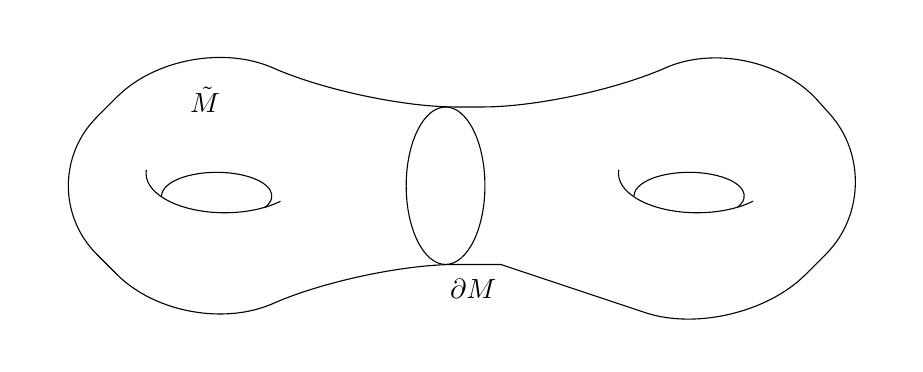
\begin{tikzpicture}
		\draw[rounded corners=35pt](6,-1)--(4.2,-1)--(2,-2)--(0,0)--(2,2)--(4.2,1)--(7,1)--(9.2,2)--(11,0)
		--(9,-2)--(6,-1);
		\draw (1.5,0.2) arc (175:315:1cm and 0.5cm);
		\draw (3,-0.28) arc (-30:180:0.7cm and 0.3cm);
		\draw (5.8,0) arc (0:360:0.5cm and 1cm);
		\draw (7.5,0.2) arc (175:315:1cm and 0.5cm);
		\draw (9,-0.28) arc (-30:180:0.7cm and 0.3cm);
		\node (a) at (-13:5.8) {$\partial M$};
		\node (a) at (26:2.5) {$\tilde{M}$};
	\end{tikzpicture}
		\caption{Variedad doble}
		\label{fig:1_04b}
	\end{subfigure}
	\caption{Ejemplo de 2 figuras}
	\label{fig:1_04}
\end{figure}


\begin{figure}[H]
	\centering
	\begin{subfigure}{0.4\textwidth}
		\centering
		\begin{tikzpicture}[scale=1.5, node distance=1.5cm and 1.8cm, 
			every node/.style={minimum size=0.8cm, inner sep=0pt}]
			
			% Definir los nodos
			\node (1) {$\{X,\emptyset\}$};
			% \node (2) [above=of 1, xshift=1.5cm] {2};
			\node (2) [above=of 1] {$\tau_{1}$};
			\node (3) [left=of 2] {$\tau_{2}$};
			\node (4) [right=of 2] {$\tau_{3}$};
			\node (5) [above=of 2, xshift=1.5cm] {$\tau_{4}$};
			\node (6) [left=of 5] {$\tau_{5}$};
			\node (7) [right=of 5] {$\tau_{6}$};
			\node (8) [left=of 6] {$\tau_{7}$};
			\node (9) [above=of 5, xshift=-1.5cm] {$\tau_{8}$};
			\node (10) [left=of 9] {$\tau_{9}$};
			\node (11) [right=of 9] {$\tau_{10}$};
			\node (12) [above=of 9] {$2^{X}$};
			
			% Dibujar las aristas (sin flechas para un diagrama de Hasse)
			\draw (1) -- (2);
			\draw (1) -- (3);
			\draw (1) -- (4);
			\draw[red, thick] (2) -- (6);
			\draw[red, thick] (2) -- (5);
			\draw (3) -- (8);
			\draw (4) -- (7);
			\draw (4) -- (5);
			\draw (8) -- (10);
			\draw[red, thick] (6) -- (10);
			\draw[red, thick] (6) -- (9);
			\draw[red, thick] (5) -- (9);
			\draw (7) -- (11);
			\draw (11) -- (12);
			\draw[red, thick] (10) -- (12);
			\draw[red, thick] (9) -- (12);
		\end{tikzpicture}
		\caption{Si $\tau_i \subseteq \tau_j$  y $\tau_i$ es Hausdorff. Entonces $\tau_j$ es Hausdorff}
		\label{fig:1_04a}
	\end{subfigure}\hfill
	\begin{subfigure}{0.4\textwidth}
		\centering
		\begin{tikzpicture}[scale=1.5, node distance=1.5cm and 1.8cm, 
			every node/.style={minimum size=0.8cm, inner sep=0pt}]
			
			% Definir los nodos
			\node (1) {$\{X,\emptyset\}$};
			% \node (2) [above=of 1, xshift=1.5cm] {2};
			\node (2) [above=of 1] {$\tau_{1}$};
			\node (3) [left=of 2] {$\tau_{2}$};
			\node (4) [right=of 2] {$\tau_{3}$};
			\node (5) [above=of 2, xshift=1.5cm] {$\tau_{4}$};
			\node (6) [left=of 5] {$\tau_{5}$};
			\node (7) [right=of 5] {$\tau_{6}$};
			\node (8) [left=of 6] {$\tau_{7}$};
			\node (9) [above=of 5, xshift=-1.5cm] {$\tau_{8}$};
			\node (10) [left=of 9] {$\tau_{9}$};
			\node (11) [right=of 9] {$\tau_{10}$};
			\node (12) [above=of 9] {$2^{X}$};
			
			% Dibujar las aristas (sin flechas para un diagrama de Hasse)
			\draw[red, thick] (1) -- (2);
			\draw (1) -- (3);
			\draw[red, thick] (1) -- (4);
			\draw[red, thick] (2) -- (6);
			\draw[red, thick] (2) -- (5);
			\draw (3) -- (8);
			\draw (4) -- (7);
			\draw[red, thick] (4) -- (5);
			\draw (8) -- (10);
			\draw (6) -- (10);
			\draw[red, thick] (6) -- (9);
			\draw[red, thick] (5) -- (9);
			\draw (7) -- (11);
			\draw (11) -- (12);
			\draw (10) -- (12);
			\draw (9) -- (12);
		\end{tikzpicture}
		\caption{Si $\tau_i \subseteq \tau_j$  y $\tau_j$ es compacta. Entonces $\tau_i$ es compacta}
		\label{fig:1_04b}
	\end{subfigure}
  \vspace{1em} % Espacio vertical entre filas

% Segunda fila: imagen centrada
\begin{subfigure}[b]{0.45\textwidth}
	\centering
	\begin{tikzpicture}[scale=2, node distance=1.5cm and 1.8cm, 
		every node/.style={minimum size=0.8cm, inner sep=0pt}]
		
		% Definir los nodos
		\node (1) {$\{X,\emptyset\}$};
		% \node (2) [above=of 1, xshift=1.5cm] {2};
		\node (2) [above=of 1] {$\tau_{1}$};
		\node (3) [left=of 2] {$\tau_{2}$};
		\node (4) [right=of 2] {$\tau_{3}$};
		\node (5) [above=of 2, xshift=1.5cm] {$\tau_{4}$};
		\node (6) [left=of 5] {$\tau_{5}$};
		\node (7) [right=of 5] {$\tau_{6}$};
		\node (8) [left=of 6] {$\tau_{7}$};
		\node (9) [above=of 5, xshift=-1.5cm] {$\tau_{8}$};
		\node (10) [left=of 9] {$\tau_{9}$};
		\node (11) [right=of 9] {$\tau_{10}$};
		\node (12) [above=of 9] {$2^{X}$};
		
		% Dibujar las aristas (sin flechas para un diagrama de Hasse)
		\draw (1) -- (2);
		\draw (1) -- (3);
		\draw (1) -- (4);
		\draw (2) -- (6);
		\draw (2) -- (5);
		\draw (3) -- (8);
		\draw (4) -- (7);
		\draw (4) -- (5);
		\draw (8) -- (10);
		\draw (6) -- (10);
		\draw (6) -- (9);
		\draw (5) -- (9);
		\draw (7) -- (11);
		\draw (11) -- (12);
		\draw (10) -- (12);
		\draw (9) -- (12);
	\end{tikzpicture}
	\caption{Teorema } 
	\label{fig:1_04c}
\end{subfigure}
	\caption{Ejemplo de 3 figuras}
	\label{fig:1_04}
\end{figure}

\section{Citas y Comandos}
\subsection{Citas y referencias}
Si tenemos un bloque tipo referencia
\defnr{Nombre de la definición con referencia}{nombre_referencia}{\lipsum[1] }
Para citar esta definición usamos \ref{def:nombre_referencia}
\subsubsection{Citar libros}
Para citar un libro del archivo ''References.bib'' usamos \cite{arnold-1989}

\subsection{Comandos}
Para escribir letras tipo conjunto
$$\RR \CC \AA \QQ \NN \II$$
Para escribir letras cursiva
$$\R \C \A \n \I$$